\documentclass[article,12pt,onesidea,4paper,english,brazil]{abntex2}

\usepackage{lmodern, indentfirst, nomencl, color, graphicx, microtype, lipsum}			
\usepackage[T1]{fontenc}		
\usepackage[utf8]{inputenc}		
\usepackage{commath}
\setlrmarginsandblock{2cm}{2cm}{*}
\setulmarginsandblock{2cm}{2cm}{*}
\checkandfixthelayout

\setlength{\parindent}{1.3cm}
\setlength{\parskip}{0.2cm}

\SingleSpacing

\begin{document}
	
	\selectlanguage{brazil}
	
	\frenchspacing 
	
	\begin{center}
		\LARGE ORIGEM E ANSEIOS DO ALUNO DO CURSO TÉCNICO EM AGROPECUÁRIA DO \\IFRO -- CÂMPUS ARIQUEMES\
		
		
		\normalsize
		Bianca Lauane Santana de Melo\footnote{Bolsista (modalidade), bnclauane@gmail.comCampus Ariquemes. } 
		Mayko da Silva Fernandes\footnote{Colaborador(a),mayko.fernandes@ifro.edu.br, Campus Ariquemes. .} \\
	Quezia da Silva Rosa\footnote{Orientador(a), quezia.rosa@ifro.edu.br, Campus Ariquemes.} 
		Fernando Alves da Silva \footnote{ Co-orientador(a), fernando.silva@ifro.edu.br, Campus Ji-Paraná.} 
	\end{center}
	
	% resumo em português
	\begin{resumoumacoluna}
	O objetivo deste artigo é identificar a origem e os anseios dos alunos do curso técnico em agropecuária do IFRO – Campus Ariquemes, pois conhecer o aluno é fundamental para o estabelecimento de práticas que auxiliem na permanência e no êxito do aluno. A pesquisa descritiva foi realizada com quarenta dos noventa e oito alunos do primeiro ano do curso Técnico em Agropecuária – Turma 2016. Foi utilizado como instrumento de coleta de dados, questionário contendo perguntas abertas e fechadas. A análise dos dados se deu através de planilhas. Os resultados apontam que o curso técnico em agropecuária do Campus Ariquemes atende prioritariamente a Região do Vale do Jamari. Os alunos do sexo masculino em sua maioria são oriundos da zona rural enquanto que as do sexo feminino são em sua maioria, provenientes da zona urbana. O prosseguimento dos estudos foi apresentado como o maior anseio dos alunos.
	
		\vspace{\onelineskip}
		
		\noindent
		\textbf{Palavras-chave}: Ensino Técnico. Perfil do aluno. Perspectivas Profissionais. 
	\end{resumoumacoluna}
	
	\section*{Introdução}
	
O Instituto Federal de Ciência e Tecnologia de Rondônia (IFRO) tem como missão “Promover educação científica e tecnológica de excelência no Estado de Rondônia voltada à formação de cidadãos comprometidos com o desenvolvimento e a sustentabilidade da sociedade” (IFRO, 2016b, p. 5). Para tanto, se faz necessário conhecer o perfil do aluno, que é a descrição de uma pessoa permitindo a identificação de dados pessoais, preferências, características, objetivos, entre outros. No ambiente educacional a descrição de perfis de alunos permite que se tenha um maior conhecimento da realidade e das necessidades do aluno,tornando o sistema mais adaptativo (PENTEADO e MARTINS, 2010). Além disso, o perfil permite a valorização do saber que o aluno traz consigo, melhor planejamento da instituição e a proposição de melhorias nas ações a serem desenvolvidas para otimizar recursos utilizados; permitirá ainda uma auto avaliação da prática docente e auxiliará na formulação de políticas relativas aos alunos (SILVEIRA, 2005).

Este trabalho objetiva analisar os alunos do curso técnico em agropecuária, apresentar seu perfil, sua origem e anseios para após o término do curso.


	
	\section*{Material e Método}
	
	O trabalho é fruto de uma pesquisa do tipo descritiva e o universo pesquisado foi composto pelos alunos ingressantes no Curso Técnico em Agropecuária do IFRO. A amostra é representada pelos alunos do primeiro ano (2016) que apresentaram Termo de Assentimento Livre e Esclarecido – TALE assinado pelos pais ou responsáveis por se tratarem de alunos menores de idade. O TALE foi entregue aos alunos na data de 23 de fevereiro de 2016 e teve como prazo final  para o recolhimento 18 março de 2016. De posse dos TALES assinados, a pesquisa foi realizada com 40 dos 98 alunos constantes na lista de frequência. A coleta de dados deu através de questionário que é um conjunto de perguntas que podem ter respostas fechadas ou abertas (ANDRADE, 2010). No questionário utilizado as perguntas foram prioritariamente fechadas, utilizando-se de questões abertas apenas para identificar a cidade de origem. A análise dos dados foi realizada através de planilhas para extração dos dados.
	
	\section*{Resultados e Discussão}
	
	Em relação ao perfil do aluno, os dados coletados apontam que 16 alunos  são do sexo masculino e 24 do sexo feminino, representando 40\% e 60\% respectivamente. Quanto à idade, os alunos respondentes têm entre 14 e 17 anos, sendo que a maioria deles, ou seja, 72\%, tem 15anos.
	No que diz respeito ao município de origem, 52\% dos alunos responderam que são do município de Ariquemes.Outros municípios do Vale do Jamari representam 33\% da procedência dos alunos. Os 15\% restantes se dividem entre outros municípios do Estado de Rondônia.
	
	Quando se avalia a procedência dos alunos, tem-se que 23 alunos vieram da zona urbana e 17 da zona rural, ou seja, 58\% e 42\% respectivamente. Quando se estratifica esses números tomando por base o sexo dos alunos, percebe-se que a maioria dos meninos, representada por 11, vieram da zona rural; enquanto que as meninas, a maioria é advinda da zona urbana num quantitativo de 18. Em suma, oriundos do campo, temos 69\% de alunos e 25\% de alunas.
	
	Quanto a isso, convém analisar a Política de Assistência Estudantil-PAE do IFRO, que tem o objetivo de ampliar as condições de permanência e êxito através  de programas que buscam permitir que tanto alunas quanto alunos oriundos da zona rural possam ingressar e permanecer no ensino técnico (IFRO,2016a).
	
	Em relação ao que pretende após a formação no curso técnico, os alunos tinham quatro possibilidades de resposta que poderiam ser combinadas entre si (gráfico 3). A maioria dos alunos pretende trabalhar e estudar, totalizando 14 alunos ou 35\%, em seguida vem os alunos que pretendem apenas estudar, com 11 alunos representando 28\%. A seguir, tem os que pretendem apenas trabalhar, esses são um total de 6 alunos, ou 15\%. Os alunos que pretendem estudar e voltar para a propriedade rural, representam 10\% do total. Alguns tencionam abrir o seu próprio negócio e estudar, esse são 3 alunos, que representam 8\%.
	\begin{figure}[h]
		\centering
		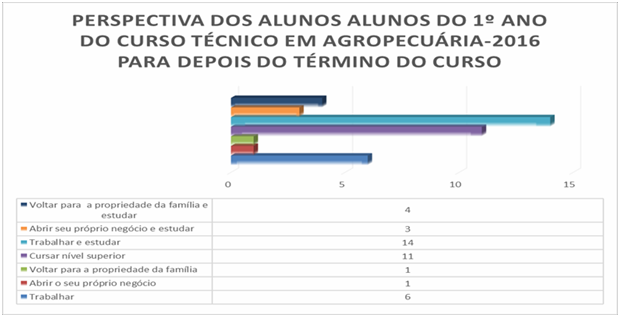
\includegraphics[width=\linewidth]{pip-artigo14-01}
		\caption{Perspectiva do aluno ao término do curso}
		\label{fig:pip-artigo14-01}
	\end{figure}
Observa-se que estudar, quer exclusivamente ou em concomitância com outras atividades, está presente em 80\% das respostas. O aluno do ensino técnico integrado se iguala ao aluno do ensino médio no que tange à importância dada ao ingresso no nível superior. Em estudo conduzido por Sparta e Gomes (2005), foi constatado que o ingresso na educação superior é a principal alternativa de escolha para o jovem que termina o ensino médio. No ensino médio a escolha é natural, no entanto, convém analisar com mais cuidado essa questão, uma vez que o ensino técnico se propõe primordialmente a capacitar o aluno a exercer uma atividade profissional após o encerramento do curso.

Outro ponto que merece atenção é que os alunos em sua maioria, não apresentam a intenção de voltar à zona rural, indicando que após terminar o curso técnico, tendem a permanecer na cidade, quer estudando, trabalhando ou ambos. Tal resultado está de acordo com o que diz Dotto (2010) que ao analisar o papel da escola na formação da identidade do jovem, identifica duas situações referentes à formação do aluno, uma é que o jovem pode converter o conhecimento obtido para o campo, aperfeiçoando as técnicas de produção e comercialização, mas ele pode também ter a ampliação das oportunidades de emprego fora do campo, e assim vislumbrar a oportunidade para deixar a penosidade do trabalho rural.

Acreditando que isso vai impactar os índices de êxodo rural do jovem e na manutenção da propriedade rural na família, o IFRO pode agir de modo a minimizar essas questões através de disciplinas, como empreendedorismo e gestão e planejamento agropecuário demonstrando a viabilidade da condução do negócio rural.
	
	\section*{Conclusões}
	
	Conclui-se que os ingressantes no curso Técnico em Agropecuária são da Região do Vale do Jamari e enquanto os homens em sua maioria são oriundos da zona rural, as alunas, em sua maioria, são oriundas da zona urbana. Independentemente de onde reside, a maioria possui propriedade rural na família. O maior anseio dos alunos é dar continuidade aos estudos,ainda que isso sedê concomitantemente com um emprego ou com o trabalho na propriedade da família. No entanto, a maioria absoluta dos alunos, indicam que não regressarão ao campo após o término do ensino técnico.
	
	Recomenda-se um estudo mais aprofundado acerca dos impactos do ensino técnico na propriedade familiar e de como o empreendedorismo pode criar alternativas para o jovem permanecer em sua propriedade gerando renda e desenvolvimento para sua região.
	
	\section*{Instituição de Fomento}
	
	IFRO – Campus Ariquemes – Departamento de Pesquisa, Inovação e Pós-Graduação.
	
	\section*{Referências}
	
\noindent ANDRADE, Maria Margarida. Introdução à Metodologia do Trabalho Científico: elaboração de trabalhos na graduação. 10. Ed. São Paulo: Atlas, 2010.


\noindent DOTTO, Fabiano. Fatores que influenciam a permanência dos jovens na agricultura familiar, no estado de Mato Grosso do Sul. 09/08/2011. 113f. Dissertação – Universidade Católica Dom Bosco. Campo Grande: 2011.


\noindent IFRO. Instituto Federal de Educação Ciência e Tecnologia de Rondônia. Plano Estratégico de permanência e êxito dos estudantes do IF Rondônia. Porto Velho: IFRO, 2016a.


\noindent \_\_\_\_\_. Instituto Federal de Educação, Ciência e Tecnologia de Rondônia. Plano de Desenvolvimento Institucional 2014 - 2018, Disponível em <http://ifro.edu.br>. Acesso em 22 abr. de 2016b.

\sloppy
\noindent PENTEADO, Fabiana. MARTINS Daniel. Agentes Pedagógicos para o ensino de Lógica com interações baseadas no perfil do aluno e em Objetos de Aprendizagens.
Disponível em:
<http://webcache.goo gleusercontent.com/search?q=cache:RFZtSfA8SBsJ:xitaocrazy.googlecode.com/svn/trunk/Mestrado/Tem a\%2520de\%2520Disserta\%25C3\%25A7\%25C3\%25A3o/Artigos/artigo\_tutor\_pedagogico\_Vrs\_06\_ 09\_2010.doc+\&cd=1\&hl=pt-BR\&ct=clnk\&gl=br\&client=firefox-b> Acesso em: 16 de mai. de 2016.


\noindent SPARTA, Mônica; GOMES, William B. Importância atribuída ao ingresso na educação superior por alunos do ensino médio. Revista Brasileira de Orientação Profissional, v. 6, n. 2, p. 45-53, 2005.


\noindent  SILVEIRA, Ricardo de Jesus. Et al. (Coord.). Perfil do aluno. Londrina: PROPLAN, 2005.

	
\end{document}